%!TEX root=seke.tex
% mainfile: ../seke.tex

\textbf{Results}. Our experiments reveal that, when doubling \texttt{UNIQUE}s, {\tt NOT NULL}s, and {\tt CHECK}s,
\textit{SchemaAnalyst} displays linear or linearithmic worst-case time complexity.  Out of the 699 experiments performed
to double these schema structures, $72\%$ converged to linear or linearithmic.  Another $8\%$ failed to converge, and of
these experiments, $80\%$ failed because of memory limitations, $13\%$ exceeded the maximum time limit, and $8\%$ failed
for reasons that could not be determined.  The doubling ratios among these experiments were primarily linear or
linearithmic at the time they were terminated, however there were $14$ that were quadratic and three that were cubic.
The experiments that failed to converge were primarily generating test data for complex schemas, such as iTrust and
BioSQL, and the most stringent adequacy criteria, such as ANCC and AUCC. The remaining $20\%$ of the 699 experiments
converged on constant or logarithmic.  Since there did not seem to be a pattern in which configurations converged this
way compared to linear or linearithmic, it is likely that they terminated before the true worst-case time complexity was
apparent.

\begin{figure}[t]
\centering
  \centering
  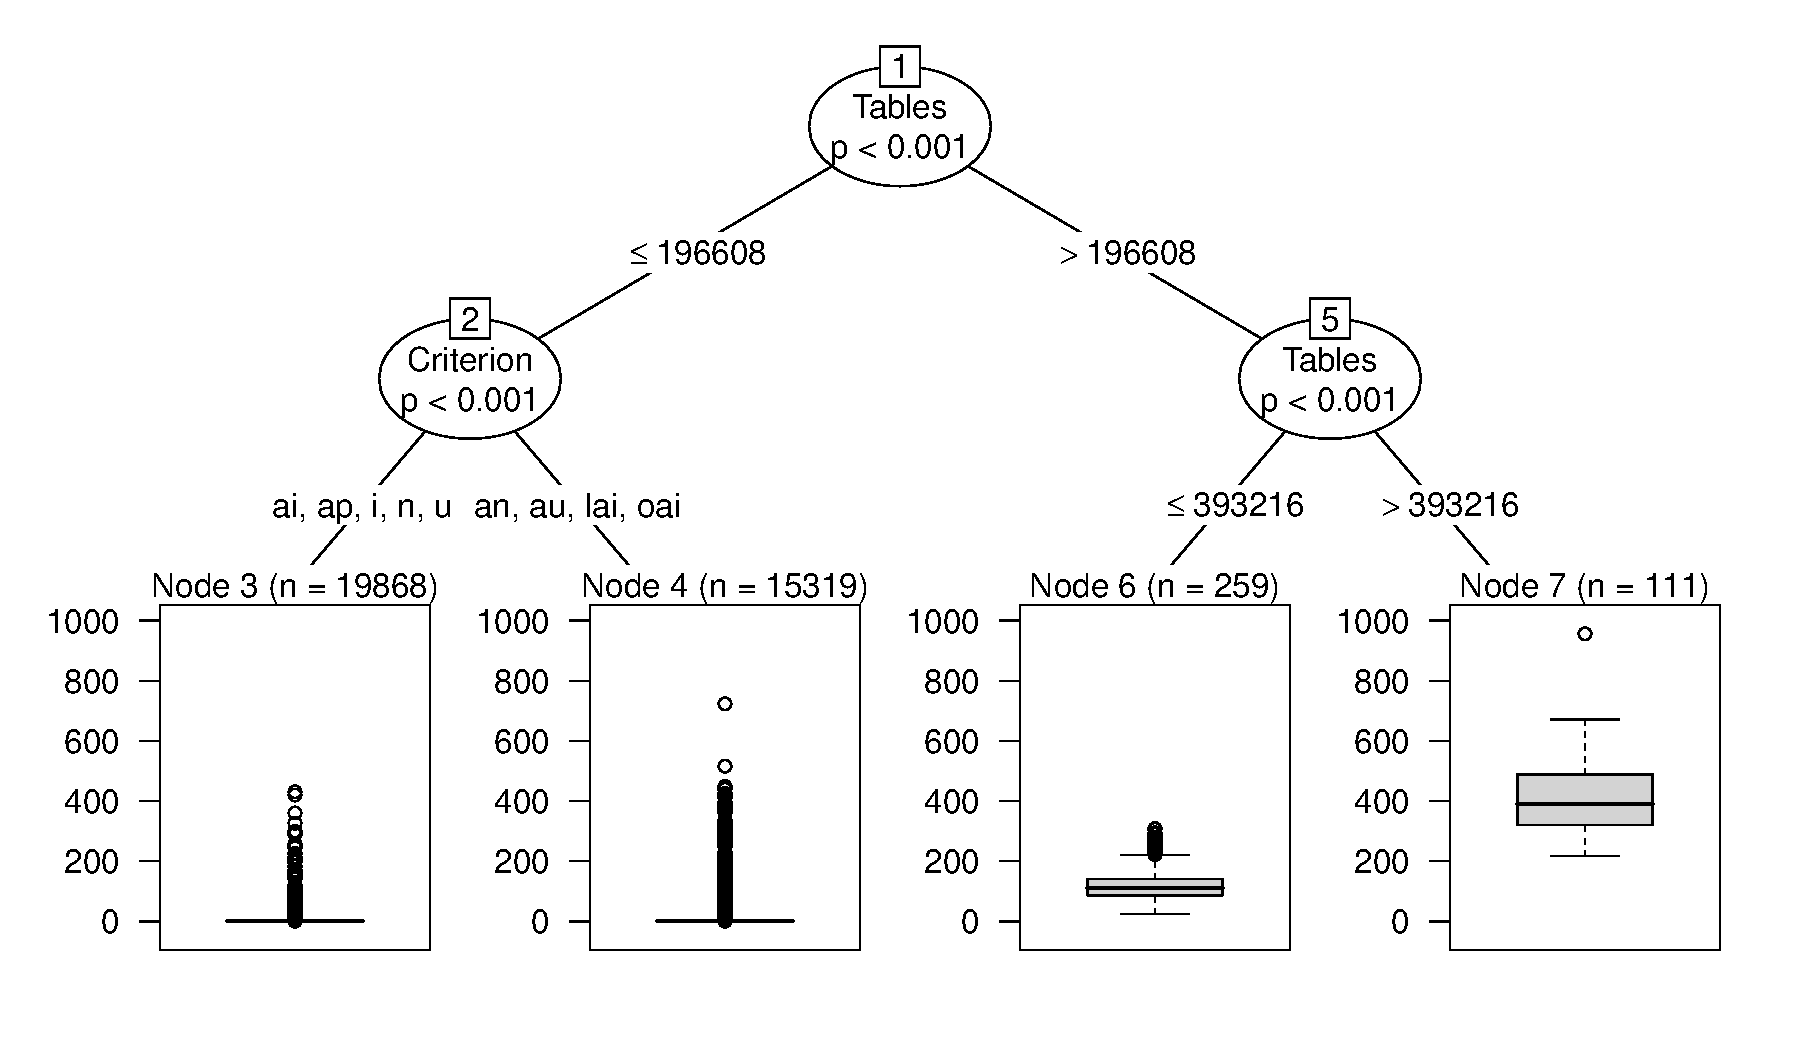
\includegraphics[width=1.025\linewidth]{diagrams/Tree.pdf}
  \vspace*{-.25in}
  \caption{Tree model using all variables to predict runtime in minutes,
  demonstrating the important of the table count. \\ Due to space
  constraints, criterion names are abreviated.
  \vspace{-.35in}}~\label{fig:atree}
\end{figure}

When doubling the tables and columns in the schemas, the results were less conclusive. Doubling the number of tables in
the schema caused the runtime of \textit{SchemaAnalyst} to increase much faster than it did for the other integrity
constraints. As a result, $56\%$ of the 467 experiments doubling this schema feature were terminated before convergence
because they exceeded the time limit.  Of the experiments that converged, 72 converged to quadratic and 10 converged to
cubic.  Of the experiments that terminated before they converged, the doubling ratios for 205 indicated quadratic, 18
suggested cubic, and 37 were worse than cubic.

Experiments on the number of columns were also inconclusive.  We noted that 208 of the converged experiments showed
linear or linearithmic time complexity, while 28 converged to quadratic and 2 cubic.  Another 203 experiments failed to
converge; however, unlike the experiments that doubled the number of tables, the experiments for doubling the number of
columns most frequently failed by running out of memory rather than exceeded the time limit. The experiments that did not
converge included 106 ratios indicating quadratic behavior, 73 cubic, and 3 worse.

% GMK NOTE: These have now been moved to another file!

% Box and whisker plots
% Belongs to results_bwplots, but must be here for positioning reasons
